\documentclass[conference]{IEEEtran}
\IEEEoverridecommandlockouts
% The preceding line is only needed to identify funding in the first footnote. If that is unneeded, please comment it out.
\usepackage{cite}
\usepackage{amsmath,amssymb,amsfonts}
\usepackage{algorithmic}
\usepackage{graphicx}
\usepackage{textcomp}
\usepackage{xcolor}
\usepackage[brazilian]{babel}
\usepackage[utf8]{inputenc}
\usepackage[T1]{fontenc}
\usepackage{listings}
\usepackage{color}
\usepackage{float}
\usepackage{multirow}
\usepackage{hyperref}

\definecolor{dkgreen}{rgb}{0,0.6,0}
\definecolor{gray}{rgb}{0.5,0.5,0.5}
\definecolor{mauve}{rgb}{0.58,0,0.82}

\lstset{frame=tb,
  language=Java,
  aboveskip=3mm,
  belowskip=3mm,
  showstringspaces=false,
  columns=flexible,
  basicstyle={\small\ttfamily},
  numbers=none,
  numberstyle=\tiny\color{gray},
  keywordstyle=\color{blue},
  commentstyle=\color{dkgreen},
  stringstyle=\color{mauve},
  breaklines=true,
  breakatwhitespace=true,
  tabsize=3
}
\lstset{language=Python}
\def\BibTeX{{\rm B\kern-.05em{\sc i\kern-.025em b}\kern-.08em
    T\kern-.1667em\lower.7ex\hbox{E}\kern-.125emX}}
\begin{document}

\title{Relatório do Laboratório 9: \\ Redes Neurais Convolucionais\\
}

\author{\IEEEauthorblockN{Isabelle Ferreira de Oliveira}
\IEEEauthorblockA{\textit{CT-213 - Engenharia da Computação 2020} \\
\textit{Instituto Tecnológico de Aeronáutica (ITA)}\\
São José dos Campos, Brasil \\
isabelle.ferreira3000@gmail.com}
}

\maketitle

\begin{abstract}
Esse relatório documenta a implementação, treino e teste da rede neural LeNet-5 usando o \textit{dataset} MNIST, que consiste num conjunto grande de imangens anotadas de dígitos decimais escritos à mão. Assim, será reproduzido um trabalho clássico da literatura de Redes Neurais Convolucionais (CNNs), que foi realizado originalmente por Yann LeCun.
\end{abstract}

\begin{IEEEkeywords}
\textit{LeNet-5}, \textit{MNIST}, Redes Neurais Convolucionais, Keras, Tensorflow
\end{IEEEkeywords}

\section{Implementação}
Para a implementação da rede neural conforme os parâmetros requisitados pelo roteiro do laboratório \cite{roteiro}, era necessário utilizar do código de adição de camadas a uma rede, fortemente inspirado das linhas de código apresentadas na seção Dicas do roteiro do laboratório \cite{roteiro}. Um detalhe importante a ser sitado foi que na criação das camadas de average pooling no Keras, os parâmetros \textit{px} e \textit{py} (no parâmetro \textit{pool\underline{\space}size}) são os tamanhos do Kernel apresentados nos requisitos para cada uma dessas camadas.

A rede então foi treinada utilizando o script \textit{train\underline{\space}lenet5.py} e os resultados desse treinamento foi exibido no \textit{Tensorboard}, mostrado a partir da execução do script \textit{run\underline{\space}tensorboard.py}. Ambos scripts já foram fornecidos previamente no código básico disponibilizado para esse laboratório.

Por fim, a rede foi avaliada no \textit{test set} usando o script \textit{evaluate\underline{\space}lenet5.py}, gerando exemplos gráficos de predições corretas e outras erradas.

\section{Resultados e Conclusões}

\subsection{Gráficos gerados no Tensorboard}
Os gráficos gerados pelo treinamento da rede e apresentados no Tensorboard foram reproduzidos nas Figuras de \ref{acc} a \ref{val_loss}.

Nas Figuras \ref{acc} e \ref{loss}, pode-se observar o aumento da acurácia no conjunto de treinamento e a diminuição na função de custo ao passar das épocas, respectivamente. Já nas Figuras \ref{val_acc} e \ref{val_loss}, esses resultados também são apresentados, mas para os conjuntos de validação. Esses comportamentos estão conforme o desejado e esperado.

\begin{figure}[htbp]
\centering
\centerline{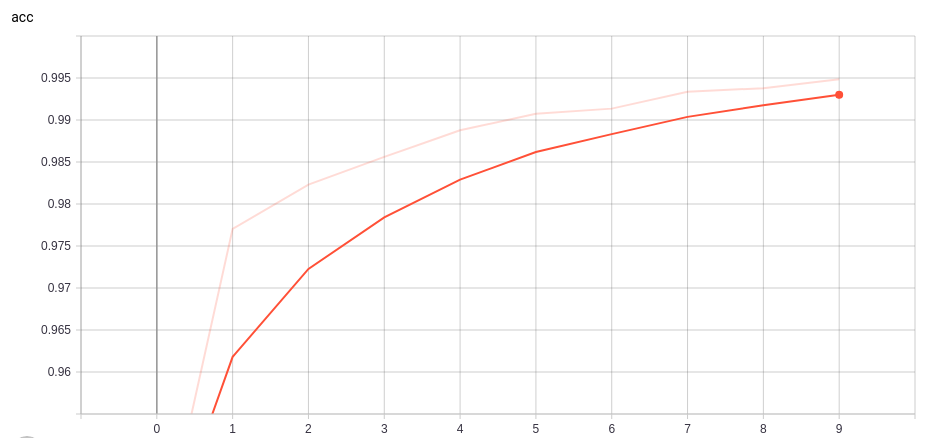
\includegraphics[scale=0.25]{imagens/acc.png}}
\caption{Acurácia do conjunto de treinamento, com o passar das épocas.}.
\label{acc}
\end{figure}

\begin{figure}[htbp]
\centering
\centerline{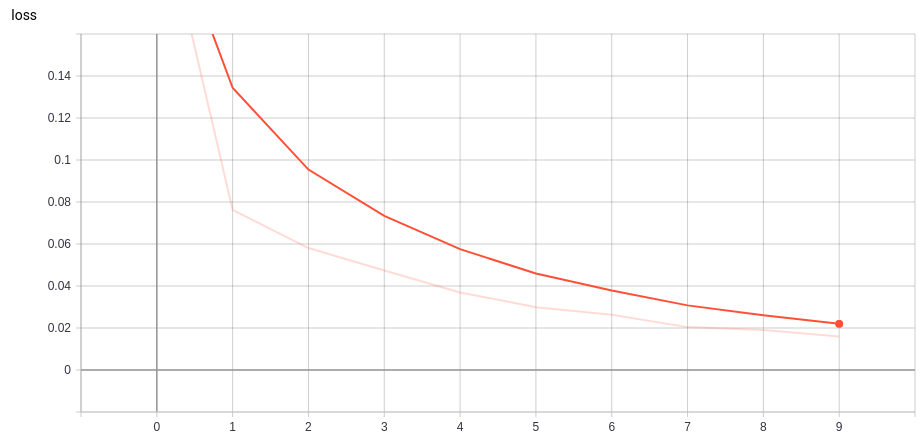
\includegraphics[scale=0.25]{imagens/loss.png}}
\caption{Custo do conjunto de treinamento, com o passar das épocas.}.
\label{loss}
\end{figure}

\begin{figure}[htbp]
\centering
\centerline{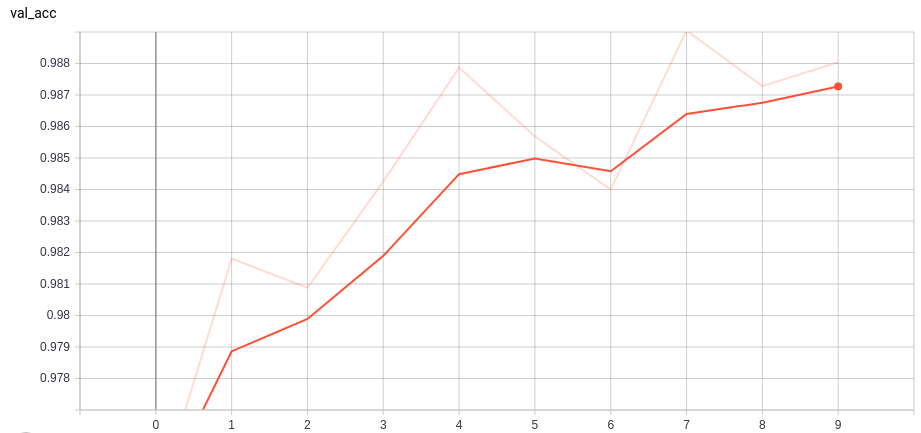
\includegraphics[scale=0.25]{imagens/val_acc.png}}
\caption{Acurácia do conjunto de validação, com o passar das épocas.}.
\label{val_acc}
\end{figure}

\begin{figure}[htbp]
\centering
\centerline{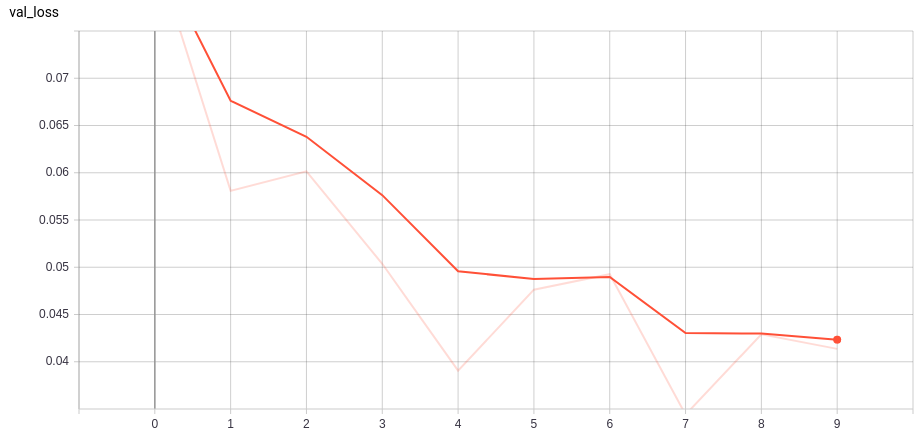
\includegraphics[scale=0.25]{imagens/val_loss.png}}
\caption{Custo do conjunto de validação, com o passar das épocas.}
\label{val_loss}
\end{figure}

\subsection{Predições realizadas pela rede}
Após a implementação e treino da rede, avaliou-se os resultados da predição para novas entradas. Algumas imagens dos resultados foram apresentadas na Figura \ref{test_image_3758} para um número manuscrito corretamente predito, e na Figura \ref{misclassified_image_8} para uma predição incorreta. Chegou-se a uma acurácia de 0.9883 nesses casos testes.

Tendo em vista o que foi apresentado, pode-se notar, por fim, que a rede neural realmente se demonstrou eficaz em realizar essa predição de números manuscritos.

\begin{figure}[htbp]
\centering
\centerline{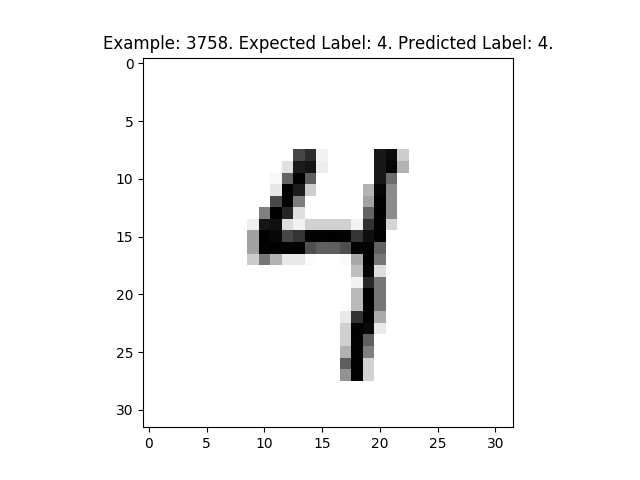
\includegraphics[scale=0.5]{imagens/test_image_3758.png}}
\caption{Número predito corretamente.}
\label{test_image_3758}
\end{figure}

\begin{figure}[htbp]
\centering
\centerline{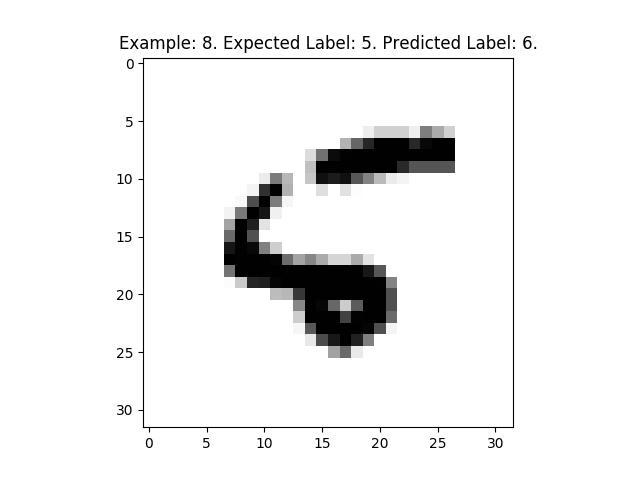
\includegraphics[scale=0.5]{imagens/misclassified_image_8.png}}
\caption{Número predito incorretamente.}
\label{misclassified_image_8}
\end{figure}

\begin{thebibliography}{00}
\bibitem{roteiro} M. Maximo, ``Roteiro: Laboratório 9 - Redes Neurais Convolucionais''. Instituto Tecnológico de Aeronáutica, Departamento de Computação. CT-213, 2019.
\end{thebibliography}

\end{document}
